\documentclass[a4paper,14pt]{extarticle} % <<< use extarticle for 14pt size

\usepackage[T2A]{fontenc}
\usepackage[utf8]{inputenc}
\usepackage[ukrainian]{babel}
\usepackage{setspace} % Optional: for nicer spacing
\usepackage{parskip} % Optional: spacing between paragraphs without indentation
\usepackage[margin=1in]{geometry}
\usepackage{graphicx}
\usepackage{array}
\usepackage{enumitem}

\usepackage{fancyhdr}
\pagestyle{fancy}
\fancyhf{}

\usepackage{amsmath}

\begin{document}
\thispagestyle{empty}

\begin{center}
    \textbf{Львівський національний університет імені Івана Франка}\\[1ex]
    Кафедра дискретного аналізу та інтелектуальних систем
\end{center}

\vspace{5cm} % Space before main title

\begin{center}
    \Large\textbf{Курс «Моделі подання знань»}\\[4ex]
    \huge\textbf{ЗВІТ}\\[3ex]
    \Large з семінарських занять за матеріалами лекцій 1-4 (пакет завдань № 1)
\end{center}

\vspace{2cm}
\begin{flushright}
    Виконав:\\
    Студент групи ПМіМ-12\\
    Паньків Олесь
\end{flushright}

\fancyfoot{Львів 2025}

\newpage
\pagestyle{plain}

\textbf{Завдання 1.} Припустімо, що агент досяг пункту, який показано на рис. 3,
а) лекції 1. (Цей рисунок тут повторено нижче.)

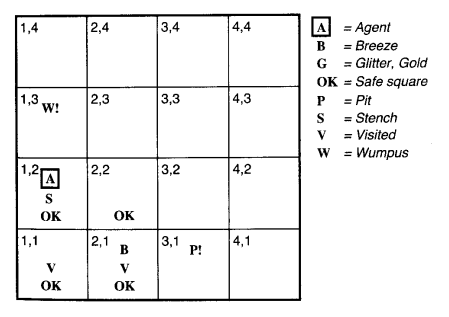
\includegraphics[width=0.6\textwidth]{resources/wampus-world-001.png}

Нехай агент отримав такі сприйняття: у квадраті [1, 1] – нічого, у квадраті [2, 1] –
вітерець, у квадраті [1, 2] – неприємний запах (на даний момент ці сприйняття утворюють
KB). На даний момент агента цікавить, що є в квадратах [1, 3], [2, 2] та [3, 1]. На основі
прикладу, наведеному на рис. 4 з лекції 2, потрібно сконструювати множину можливих
світів. (Має бути знайдено 32 таких можливих світи. Кожний з них може містити яму, і,
щонайбільше, в одному з них може перебувати вампус.) Позначте світи, у яких KB є
істинною, а також ті у яких істинним є кожне з наступних висловлень:

$\alpha_2$ = "У квадраті [2, 2] немає ями"

$\alpha_3$ = "У квадраті [1, 3] є вампус"

На основі цього доведіть, що $KB \models \alpha_2$ та $KB \models \alpha_3$.

\textbf{Розв'язок}: На основі заповненої таблиці легко дати відповіді на
сформульовані вище запитання:

\begin{tabular}{|p{0.25\textwidth}|p{0.25\textwidth}|p{0.25\textwidth}|p{0.25\textwidth}|}
\hline
\textbf{Model} & \textbf{KB} & $\alpha_2$ & $\alpha_3$ \\
\hline
& & true & \\
$P_{1,3}$ & & true & \\
$P_{2,2}$ & & & \\
$P_{3,1}$ & & true & \\
$P_{1,3}, P_{2,2}$ & & & \\
$P_{2,2}, P_{3,1}$ & & & \\
$P_{3,1}, P_{1,3}$ & & true & \\
$P_{1,3}, P_{3,1}, P_{2,2}$ & & & \\
\hline
$W_{1,3}$ & & true & true \\
$W_{1,3}, P_{1,3}$ & & true & true \\
$W_{1,3}, P_{2,2}$ & & & true \\
$W_{1,3}, P_{3,1}$ & true & true & true \\
$W_{1,3}, P_{1,3}, P_{2,2}$ & & & true \\
$W_{1,3}, P_{2,2}, P_{3,1}$ & & & true \\
$W_{1,3}, P_{3,1}, P_{1,3}$ & & true & true \\
$W_{1,3}, P_{1,3}, P_{3,1}, P_{2,2}$ & & & true \\
\hline
$W_{3,1}$ & & true & \\
$W_{3,1}, P_{1,3}$ & & true & \\
$W_{3,1}, P_{2,2}$ & & & \\
$W_{3,1}, P_{3,1}$ & & true & \\
$W_{3,1}, P_{1,3}, P_{2,2}$ & & & \\
$W_{3,1}, P_{2,2}, P_{3,1}$ & & & \\
$W_{3,1}, P_{3,1}, P_{1,3}$ & & true & \\
$W_{3,1}, P_{1,3}, P_{3,1}, P_{2,2}$ & & & \\
\hline
$W_{2,2}$ & & true & \\
$W_{2,2}, P_{1,3}$ & & true & \\
$W_{2,2}, P_{2,2}$ & & & \\
$W_{2,2}, P_{3,1}$ & & true & \\
$W_{2,2}, P_{1,3}, P_{2,2}$ & & & \\
$W_{2,2}, P_{2,2}, P_{3,1}$ & & & \\
$W_{2,2}, P_{3,1}, P_{1,3}$ & & true & \\
$W_{2,2}, P_{1,3}, P_{3,1}, P_{2,2}$ & & & \\
\hline
\end{tabular}

\newpage
\textbf{Завдання 5.} Доведіть наступні твердження:

\begin{enumerate}[label=]
    \item а) $\alpha$ загальнозначима тоді і тільки тоді, коли $True \models \alpha$.
    \item б) Для будь-якого $\alpha$, $False \models \alpha$.
\end{enumerate}

\textbf{Розв'язок}:
\begin{enumerate}[label=]
    \item а) Формула $\alpha$ є валідною тоді й тільки тоді, коли вона випливає з істини
        ($True \models \alpha$). Це значить, що якщо $\alpha$ істинна у всіх моделях,
        то вона випливає з $True$.
    \item б) Для будь-якої формули $\alpha$ виконується: $False \models \alpha$, бо брехня
        не має жодної моделі, а значить, з неї можна "вивести" все, що завгодно.
\end{enumerate}

\vspace{1cm} % Space before main title
\textbf{Завдання 9.} Використавши метод за Вашим вибором, доведіть кожну з
еквівалентностей з лістингу 4 лекції 3. (Цей Лістинг повторено нижче.)
\begin{enumerate}[label=]
    \item д) $(\alpha \implies \beta) \equiv (\neg \beta \implies \neg \alpha)$ контрапозиція
\end{enumerate}

\textbf{Розв'язок}:
\begin{enumerate}[label=]
    \item д) Розглянемо окремо ліву та праву частини:
\[
\begin{aligned}
(\alpha \rightarrow \beta) &\equiv (\neg \alpha \lor \beta) \\
(\neg \beta \rightarrow \neg \alpha) &\equiv (\neg \neg \beta \lor \neg \alpha) \equiv (\beta \lor \neg \alpha)
\end{aligned}
\]

Оскільки \((\neg \alpha \lor \beta) \equiv (\beta \lor \neg \alpha)\) за комутативністю диз'юнкції, отже:
\[
(\alpha \rightarrow \beta) \equiv (\neg \beta \rightarrow \neg \alpha)
\]
\end{enumerate}

\end{document}
